\section{Introduction}
I have spent the majority of my time this week taking part in the Media Memorability challenge from MediaEval 2018 with my teammate.

\section{Feature Extracting}
\subsection{From Video to Frames}
With 10,000 videos from the whole dataset, I used \emph{ffmpeg} to extract frame by frame of each video; as the result, I got about 80,000 frames (images) from the dataset. At the beginning, I just only extracted 3 main frames of a video at 3 time intervals (beginning, middle amd end),  but since the length of a video was only about 8 seconds, l so I decided to extract all 8 frames (1 frame per second).

This was the command line which I used to extract frames from a video. \textbf{\emph{ffmpeg -i video1.mp4 -r 1 video1-\%02d.jpg}}. The \textbf{\emph{-i}} indicated input file; \textbf{\emph{-r}} was the number of frames per second I wanted to extract (e.g. \emph{-r 1} meant 1 frame per second,  \emph{-r 0.1} meant 1 frame every 10 seconds); and the term \textbf{\emph{\%02d}} was used by \textbf{\emph{ffmpeg}} to name the output frames.

\subsection{Using TensorHub}
TensorFlow\cite{tensorflow} provided TensorHub which was a library for reusable ma-chine learning modules. TensorHub maintained several modules to extract image feature vectors like Inception, MobileNet, ResNet and DenseNet.

I successfully extracted images' features but the result stucked in the vari-ables themselves and I could not write those values to text files or numpy pickles. According to my research, I had to construct my code in a TensorFlow session to read those values, but I still got tons of errors by TensonFlow.

I would have to learn more about how to use TensorFlow correctly and try my luck again.

\subsection{Using PyTorch}
According to the comparison graph by TowardDataScience, I chose ResNet50 and Inception v3 to extract image feature because of their acceptable ratio of accuracy to complexity.

The length of feature vector of both ResNet and Inception v3 was 2048. For each video there was a corresponding numpy file ( \textbf{\emph{.npy}}) containing a 2d numpy array of size [8, 2018]. In order to load the numpy file into variable to perform computiation, I used \textbf{\emph{video = numpy.load(filename)}}; and \textbf{\emph{input = numpy.stack(input, video)}} to concatenate multiple videos into one 3d array of size [8000, 8, 2048]. The concatenation was not expensive at all because it took only 5 seconds to concatenate 8,000 videos (avoid using git \textbf{\emph{torch.cat()}} due to its poor performance).

\newpage
\begin{figure}[!ht]
\centering
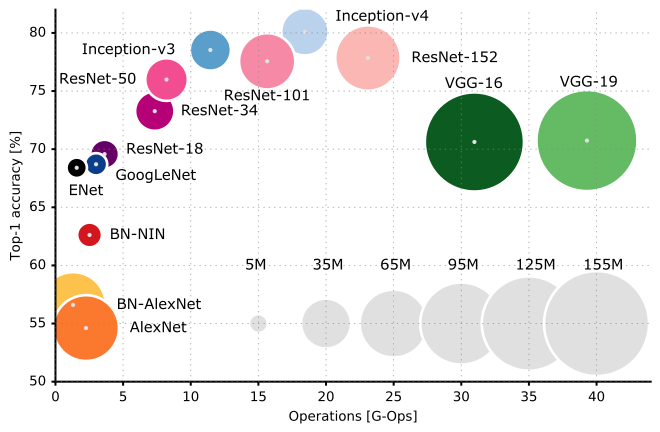
\includegraphics[width=\textwidth]{week9-cnn-architectures.png}
\caption{In-depth analysis and comparison of all networks\cite{cnnarchitectures}}
\end{figure}

\section{Evaluation Metrics}
\subsection{Pearson Correlation Coefficient}
One of the three evaluation metrics proposed by MultiMediaEval was Pear-son Correlation Coefficient. It was the measure of the linear correlation between two variables X and Y. It had a value between +1 and -1, where 1 was total positive linear correlation, 0 was no linear correlation, and -1 was total negative linear correlation. Pearson correlation coefficient was the covariance of the two variables divided by the product of their standard deviations.

\begin{figure}[!ht]
\centering
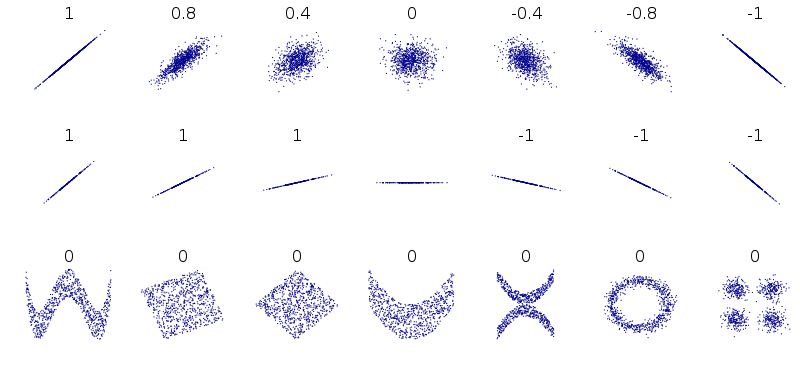
\includegraphics[width=\textwidth]{week9-pearson-example.png}
\caption{Pearson Correlation Coefficient of x and y for several (x, y) sets}
\end{figure}

\subsection{Spearman's Rank Correlation Coefficient}
The second evaluation metrics proposed was the Spearman's Rank Cor-relation Coefficient. It assessed how well the relationship between two variables could be described using a monotonic function. The Spearman correlation between two variables would be high when observations had a similar rank between the two variables, and low when observations have a dissimilar (or fully opposed for a correlation of −1) rank between the two variables. The Spearman correlation between two variables was equal to the Pearson correlation between the ranked values of those two variables; while Pearson's correlation assessed linear relation-ships, Spearman's correlation assessed monotonic relationships. The term ranked variables refered to the data transformation in which numerical or ordinal values were replaced by their rank when the data were sorted (e.g. given the numerical data 3.4, 5.1, 2.6, 7.3; the ranks of these data items would be 2, 3, 1 and 4 respectively).

\begin{figure}[!ht]
\centering
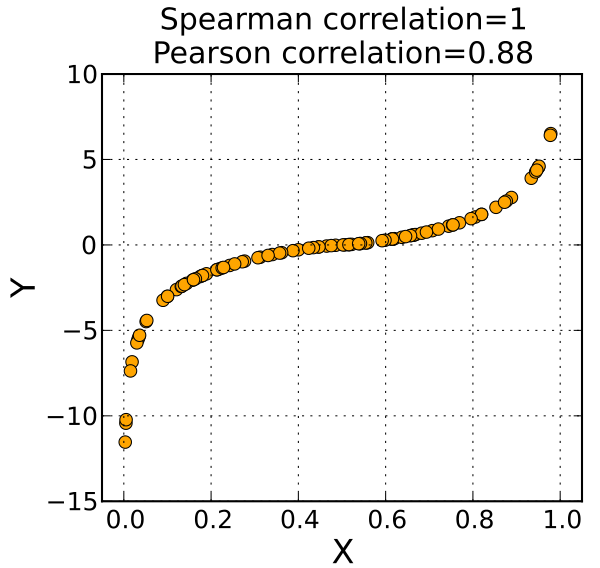
\includegraphics[width=0.5\textwidth]{week9-spearman-example.png}
\caption{Spearman Correlation Coefficient of 1}
\end{figure}

\subsection{Mean-Squared Error}
The last evaluation metric was the Mean-Square Error between two variables. I did not think this metric could be helpful for my approaches.

\subsection{Scipy Stats}
Both Spearman's Rank Correlation Co-efficient and Pearson Correlation Coefficient were supported by Scipy.Stats. The usage of each metric could be found \href{https://docs.scipy.org/doc/scipy/reference/generated/scipy.stats.spearmanr.html}{here} and \href{https://docs.scipy.org/doc/scipy-0.14.0/reference/generated/scipy.stats.pearsonr.html}{here}.

\subsection{Initiative}
After learning about Spearman's Rank Correlation Coefficient, I figured out that I did not need to compute the memorability score for each video in this challenge. Another potential approach was to sort the video list for its memorability. For example, given three videos A, B and C with theirs grouth truth memorability score of \textbf{\emph{[0.2, 0.9, 0.4]}}; I had to generate a list of ranking in term of their memorability starting with the lowest one which was \textbf{\emph{[1, 3, 2]}}. Computing Spearman's Rank Correlation Coefficient on \textbf{\emph{[0.2, 0.9, 0.4]}} and \textbf{\emph{[1, 3, 2]}} would give me the correlation of \textbf{\emph{1.0}}, which was the best score of this metric.

\section{LSTM Network on Extracted Features}
\subsection{Architecture}
I first try to connect one Long - Short Term Memory\cite{lstm} cell with one fully-connected layer to classify between 2 classes. According to an example from PyTorch, they preferred training the network sample by sample, so I tried to do that too. And the network worked, so I tried to stack 8 Long - Short Term Memory cells to test (I thought that I had 8 images per video, so stacking 8 Long - Short Term Memory cells a time was a good choice). The figure below almost demonstrated correctly what I had done so far; the key difference was that at the final <end> gate, I also added one fully-connected layer of size [2048, 2] as a classifier.

\begin{figure}[!ht]
\centering
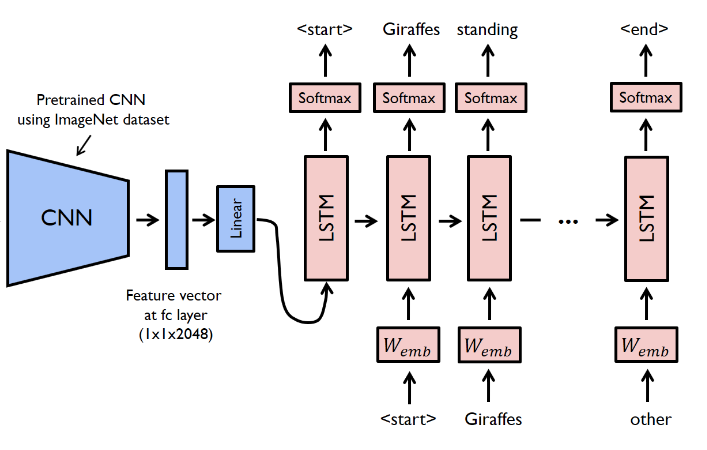
\includegraphics[width=\textwidth]{week9-lstm-network.png}
\caption{Long - Short Term Memory Network}
\end{figure}

In training process, there were some key differences such as I need to clear out the gradients before each input video (using \emph{model.zero\_grad()}) because PyTorch accumulated them. And I also need to clear out the hidden state of the Long - Short Term Memory, to detach the cell from its history on the last input video.

\subsection{Problems}
This was the first time I worked with Long - Short Term Memory cells. Although I had already obtained the main idea of Long - Short Term Memory, but in PyTorch I was so confused with the Long - Short Term Memory stacking, training, designing techniques. And I did not know how to evaluate my network, whether it was right or wrong, did I violate any rules or would it work effectively as I expected.

I did not think that my network was reliable. One epoch costed so much time, about 2.5 minutes, so if I wanted to train my network with 300 epochs it would take me 12.5 hours. I had trained my network for 150 epochs until Colab shut my session down. And even though after 150 epochs, I still got a 5-digit loss number (around 22,000).